\chapter{Stato dell'Arte}
\section{Sistemi Ferroviari e Ferrotramviari}
Il concetto di \emph{treno} come comunemente percepito nasce con l'inizio della Rivoluzione Industriale, avvenuta tra il \emph{XVIII} e il \emph{XIX} secolo, a seguito della quale l'avvento della macchina a vapore ha permesso all'umanit\`a di disporre di fonti di energia sufficienti a fare evolvere i primi rudimentali trasporti su binario negli odierni sistemi ferroviari.\\*
\noindent\`E possibile schematizzare un Sistema Ferroviario, o Ferrotramviario, come un veicolo, il treno, vincolato a muoversi attraverso una propulsione, elettrica o a combustibile, lungo una traccia fissa, il binario.\\*
Queste caratteristiche accomunano qualsiasi sistema di trasporto ferroviario o ferrotramviario a prescindere dalla sua scala in termini di veicoli transitanti ed estensione geografica. Ci\'o che invece differenzia un Sistema Ferroviario da un Sistema Ferrotramviario sono:
\begin{itemize}
	\item Le caratteristiche fisiche del treno, come lunghezza e massa;
	\item Le caratteristiche geografiche dell'ambiente operativo;
	\item Gli scopi del trasporto.
\end{itemize}
In generale, nel trasporto ferroviario si utilizzano treni caratterizzati da grandi dimensioni, che trasportano persone o merci su lunghe percorrenze (regionali, nazionali o internazionali), operando pertanto prevalentemente in ambienti extra urbani. Un esempio di treno operante in un sistema ferroviario classico \`e quello in figura \ref{fig:frecciarossa}.\\*
\begin{figure}[h]
	\centering
	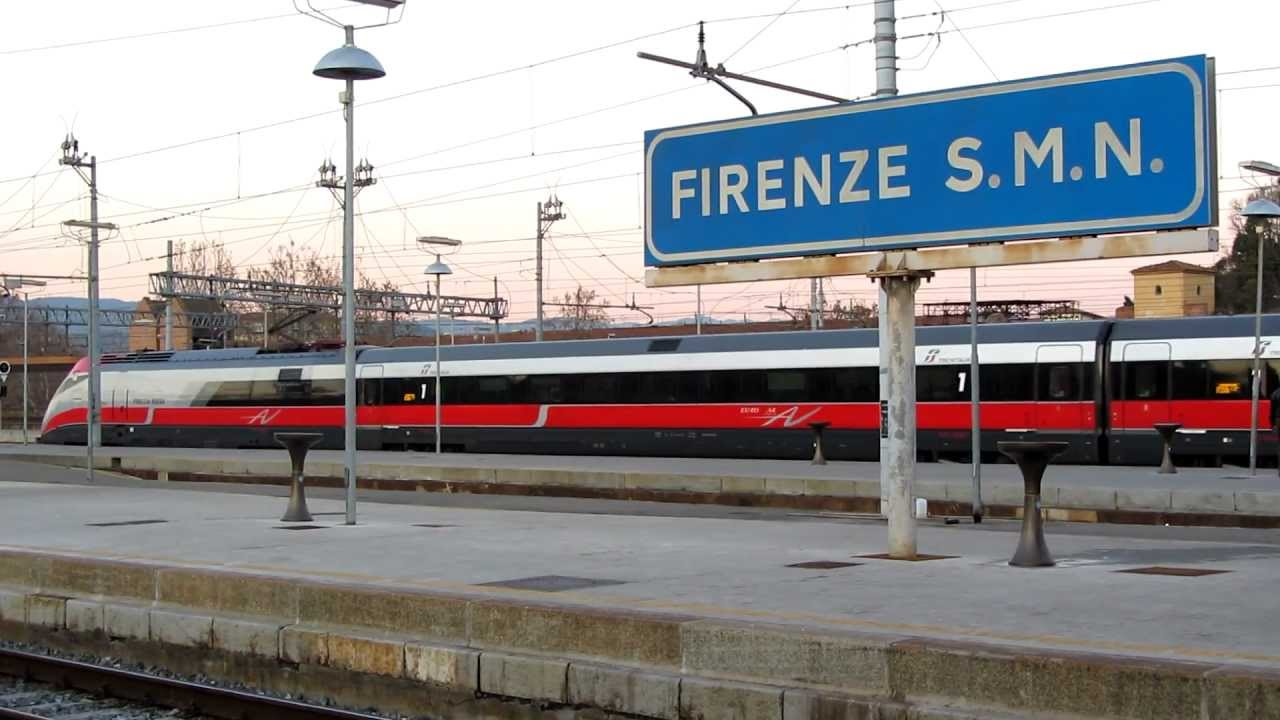
\includegraphics[width=0.7\linewidth]{img/frecciarossa}
	\caption{Treno in arrivo alla stazione ferroviaria di Firenze Santa Maria Novella}
	\label{fig:frecciarossa}
\end{figure}
Il trasporto ferrotramviario, di contro, vede l'utilizzo di treni dalle ridotte dimensioni, pi\'u leggeri di quelli usati nei sistemi ferroviari, e che hanno lo scopo di rappresentare un'alternativa per il cittadino all'utilizzo di mezzi privati durante i suoi spostamenti all'interno di un'area metropolitana. Quest'ultima caratteristica implica che l'ambiente operativo di un sistema ferrotramviario sia radicalmente diverso da quello di un sistema ferroviario: i treni si muovono lungo rotaie installate su strade urbane, quindi il traffico ferrotramviario \`e fuso con il traffico automobilistico, motociclistico, ciclistico e pedonale che caratterizza l'ambiente urbano, come mostrato nelle figure \ref{fig:danhai} e \ref{fig:tramschema}.\\*
\begin{figure}[h]
	\centering
	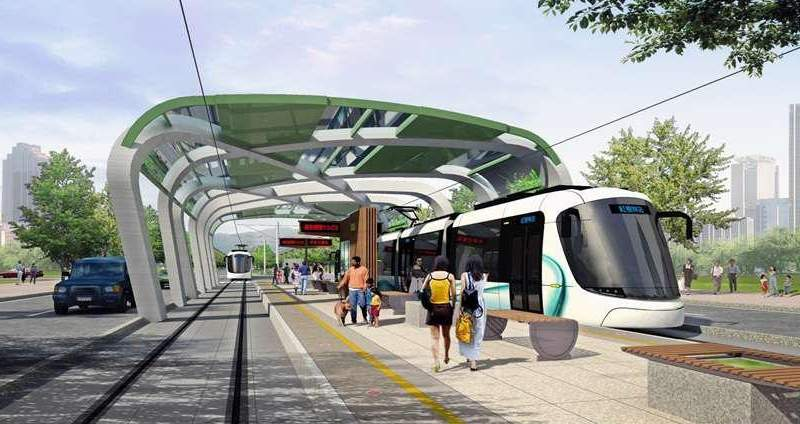
\includegraphics[width=0.7\linewidth]{img/danhai}
	\caption{Tramvia di Danhai, Taipan}
	\label{fig:danhai}
\end{figure}
\begin{figure}[h]
	\centering
	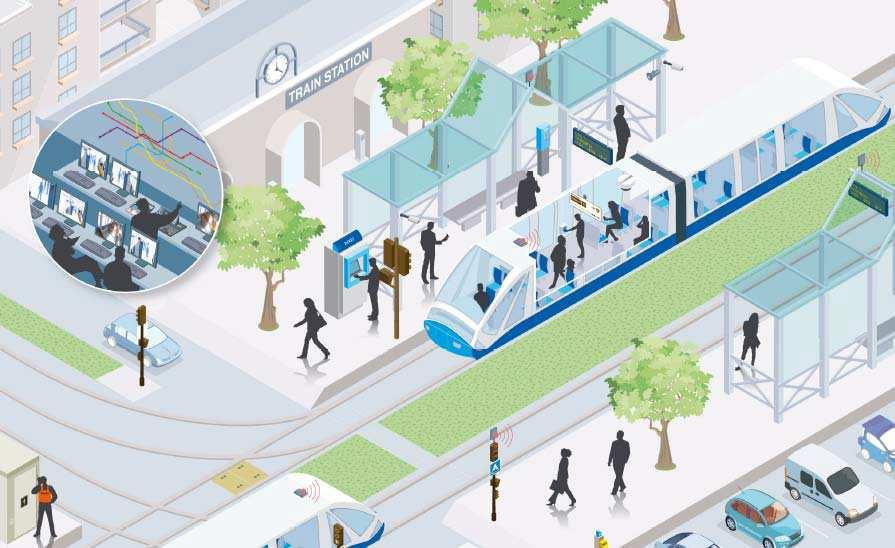
\includegraphics[width=0.7\linewidth]{img/twschema}
	\caption{Schema di un tipico scenario tramviario}
	\label{fig:tramschema}
\end{figure}
\section{Il Problema del Posizionamento}
Per posizionamento ferroviario, si intende la stima della posizione di un treno all'interno di una traccia ferroviaria. Esso esiste tanto nel contesto ferrotramviario quanto nel contesto ferroviario classico.\\*
Sovente questa stima viene espressa come progressiva chilometrica rispetto all'origine della linea oppure, pi\'u raramente, come coordinata geografica.\\*
Il problema del posizionamento sorge nel momento in cui, per ragioni di rotta, un treno ha necessit\`a di spostarsi da una sezione di binario, anche detta traccia, ad un'altra. Questa operazione di scambio \`e offerta dal sistema di \emph{interlocking}. Tale sistema \`e detto \emph{safety-critical}, in quanto offre una funzionalit\`a che deve rispettare adeguati standard di sicurezza.\\*
Gli odierni sistemi di posizionamento si basano principalmente sull'utilizzo di strumenti installati a terra, che hanno lo scopo di rilevare il passaggio di un treno, e quindi di interagire con il sistema di \emph{interlocking} della traccia al fine di garantire, con un elevato livello di confidenza, un transito sicuro dei mezzi.
\subsubsection{Odierne Tecniche di Posizionamento}
I sistemi di posizionamento attualmente in uso sono basati su un'architettura distribuita composta dai seguenti blocchi:
\begin{itemize}
	\item Sottosistema di \emph{interlocking};
	\item Sottosistema di comunicazione \texttt{treno-traccia};
	\item Sottosistema semaforico.
\end{itemize}
\paragraph{Sottosistema di interlocking:}
Il sottosistema di \emph{interlocking} \`e la parte che si fa effettivamente carico di offrire al treno un attraversamento sicuro di una \emph{Junction Area (JA)}. Una JA \`e un punto della linea ferroviara in cui il treno pu\'o cambiare direzione, e occupare una nuova traccia di binario.\\*
La nuova traccia da occupare potrebbe avere particolari vincoli sul numero di treni contemporaneamente transitanti, ed in ogni caso lo scambio di rotaia deve essere corretto ed avvenire in sicurezza, in quanto occupare la traccia sbagliata potrebbe avere ripercussioni finanche catastrofiche.\\*
Un sistema di \emph{interlocking} \`e composto dai seguenti elementi:
\begin{itemize}
	\item \emph{Switch Control Unit (UCS)}:\\*
	Piattaforma certificata \texttt{SIL-3} che rappresenta il nucleo del sistema di \emph{interlocking} e che implementa l'intera logica di gestione di una JA. Un UCS dispone di un'interfaccia di \emph{Input/Output} (I/O) verso gli elementi di \emph{interlocking} installati a terra che ne consente un controllo sicuro in accordo allo standard \texttt{SIL-3}.
\begin{figure}[h]
		\centering
		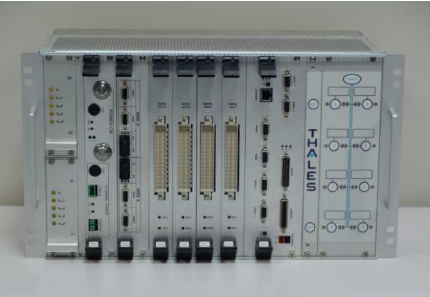
\includegraphics[width=0.7\linewidth]{img/ucs}
		\caption{UCS realizzato da Thales Italia SPA}
		\label{fig:ucs}
\end{figure}
	\item Conta Assi:\\*
	Il Conta Assi, o in inglese \emph{Axle Counter} (AC), \`e un sistema certificato \texttt{SIL-3} che ha lo scopo di rilevare la presenza del treno e fornire quindi lo stato di occupazione della sezione di traccia in cui l'AC \`e installato.
\begin{figure}[h]
	\centering
	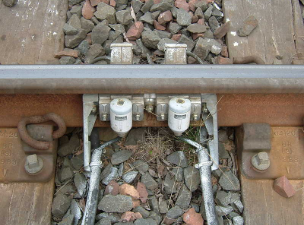
\includegraphics[width=11cm,height=3.1cm]{img/axlecounter}
	\caption{Conta Assi}
	\label{fig:ac}
\end{figure}
	\item \emph{Point Machines}:\\*
	Le \emph{Point Machines} infine, sono degli strumenti certificati \texttt{SIL-3} che hanno lo scopo di direzionare le rotaie verso una determinata sezione di traccia.
	\begin{figure}[h]
		\centering
		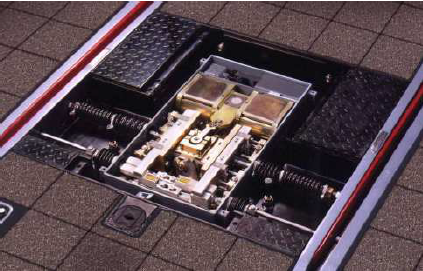
\includegraphics[width=0.7\linewidth]{img/pointmachine}
		\caption{Esempio di \emph{Point Machine} installata su una traccia ferrotramviaria}
		\label{fig:pointmachine}
	\end{figure}
\end{itemize}
L'intero sistema di \emph{interlocking} viene attivato dai \emph{Track Circuit}. Questi apparati sono installati a terra prima di ciascuna JA, e segnalano al sistema di \emph{interlocking} l'avvicinamento di un treno alla successiva JA.
\paragraph{Sottosistema di comunicazione treno-traccia:} Il sottosistema di comunicazione treno-traccia \`e gestito da un computer installato bordo treno, chiamato \emph{On Board Control Unit} (OBCU), ed ha lo scopo di fornire funzionalit\`a non legate alla \emph{safety} e pertanto poco interessanti. OBCU viene principalmente utilizzato per monitorare lo stato del traffico ferrotramviario in una architettura di \emph{monitoring} centralizzata. Il monitoring si basa su comunicazioni \emph{wireless}. In alcune applicazioni pu\'o comprendere una comunicazione pi\'u o meno diretta con il sistema di \emph{interlocking} allo scopo di segnalare l'avvicinamento del treno a una JA.
\paragraph{Sottosistema semaforico:} 
Il sottosistema semaforico prende in ingresso informazioni dal sistema di \emph{interlocking} ed eventualmente, da OBCU, e gestisce i segnali luminosi da mostrare sui semafori a un macchinista che si appresta a superare una JA.\\*In tabella \ref{tab:sem} viene riportata la lista dei segnali semaforici utilizzati nel contesto ferrotramviario.
\begin{table}
\begin{tabular}{|c|c|c|}
	\hline 
	\textbf{Segnale} & \textbf{Descrizione} & \textbf{Significato} \\

	\hline
	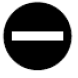
\includegraphics{img/stopsemaphore}& Barra bianca orizzontale & Fermarsi \\ 
	\hline 
	
\includegraphics{img/gosemaphore}& Barra bianca verticale  & Procedere avanti \\ 
	\hline 
	
\includegraphics{img/rightsemaphore}& Barra bianca ruotata di 45 gradi & Procedere solo a destra \\ 
	\hline 
	
\includegraphics{img/leftsemaphore}& Barra bianca ruotata di -45 gradi & Procedere solo a sinistra \\ 
	\hline 
\end{tabular} 
\caption{Segnalazioni semaforiche ferrotramviarie}
\label{tab:sem}
\end{table}
\subsection{Criticit\`a}
Le attuali tecniche di posizionamento richiedono un intervento trascurabile di computer installati a bordo e una grande quantit\`a di apparati installati a terra. Mentre i computer di bordo non forniscono in generale funzionalit\`a legate alla \emph{safety}, gli apparati installati a terra sono costosi e hanno un impatto ambientale non trascurabile.\\*
\`E possibile considerare il treno e il computer di bordo come un unico sistema, ossia il treno viene modellato come un \emph{Cyber-Physical System}.\\*
Un \emph{Cyber-Physical System} (CPS) \`e un sistema composto da una parte \emph{fisica} e da una parte \emph{cyber}. Il sottosistema fisico \`e composto da sensori e attuatori che hanno rispettivamente lo scopo di rilevare lo stato dell'ambiente circostante e di alterarlo se necessario. Il sottosistema \emph{cyber} \`e essenzialmente un elaboratore, che dispone di processore, memoria, e interfacce I/O verso i sensori gli attuatori, ed eventuali operatori  umani. Una tale architettura di sistema, permette di sfruttare le capacit\`a di calcolo dei moderni processori per implementare algoritmi anche molto complessi per il \emph{processing} di grandi quantit\`a di dati provenienti dai sensori.\\*
Lo scopo della Tesi \`e quello di mostrare il funzionamento di un possibile sistema di posizionamento alternativo al sistema tuttora operante, che sfrutti l'uso combinato di un insieme di sensori i cui dati rilevati vengono processati da un algoritmo noto come \emph{Sensor Fusion Algorithm} (SFA).\\*
\begin{figure}[h]
	\centering
	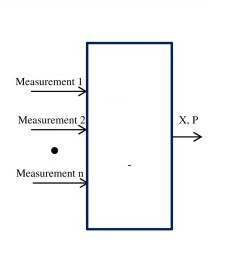
\includegraphics{img/sfaschema}
	\caption{Schema SFA}
	\label{fig:sfa}
\end{figure}
\\*
Tale algoritmo \`e schematizzabile come una \emph{black-box}: le misurazioni dei sensori sono l'ingresso, mentre l'uscita \`e la misura cercata, nella fattispecie, la posizione del treno lungo la traccia.
Utilizzando SFA, il treno \`e in grado di auto-posizionarsi, capacit\`a che minimizza la necessit\`a di installare apparati di terra.\\*
Un algoritmo che tiene conto delle misurazioni di un \emph{set} di sensori, usato in luogo di un semplice \emph{processing} di insiemi di misure provenienti da sorgenti omologhe, permette al sistema di correggere il rumore che disturba le singole misurazioni, realizzando cos\`i una nuova misura pi\`u accurata di quella che si avrebbe considerando i sensori in maniera mutuamente esclusiva.